	\begin{figure}[H]
		\centering
 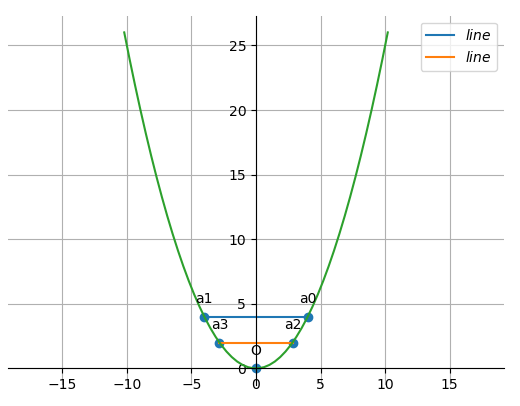
\includegraphics[width=0.75\columnwidth]{chapters/12/8/3/3/figs/conic.png}
		\caption{}
		\label{fig:12/8/3/3}
  	\end{figure}
The conic parameters are
\begin{align}
	\vec{V} = \myvec{1 & 0\\0 & 0},
	\vec{u} = \myvec{0\\-2},
	f = 0
	%\\
\end{align}
The vector parameters of 
$y-4=0$
are
\begin{align}
	\vec{h}_1=\myvec{0\\4},
	\vec{m}_1=\myvec{1\\0}
\end{align}
Substituting the above in \eqref{eq:tangent_roots},
\begin{align}
\kappa_i=4,-4
\end{align}
yielding
the points of intersection with the parabola as
\begin{align}
\vec{a}_0=\myvec{4\\4},
\vec{a}_1=\myvec{-4\\4}
\end{align}
Similarly, for 
the line $y-2=0$, the vector parameters are
\begin{align}
\vec{h}_2=\myvec{0\\2},
\vec{m}_2=\myvec{1\\0}
\end{align}
yielding 
\begin{align}
\kappa_i=2.8,-2.8
\end{align}
and the points of intersection
\begin{align}
\vec{a}_2=\myvec{2.8\\2},
\vec{a}_3=\myvec{-2.8\\2}
\end{align}
From 
		\figref{fig:12/8/3/3},
the area of the parabola between the lines $y=2$ and $y=4$ is given by
\begin{align}
\int_{0}^{4} \ 2\sqrt{y} \,dy-\int_{0}^{2} \ 2\sqrt{y} \,dy
=6.895 
\end{align}
